% ============================================================
%  CHAPTER 9: RESULTS AND DISCUSSION
% ============================================================

\chapter{RESULTS AND DISCUSSION}
\label{chap:results}

\section{Binary Packaging and Artifact Verification}
\label{sec:build_results}

The Android mobile client application was compiled, verified, and packaged into production Application Packages (APKs) targeting the \texttt{com.quantumsafe.vpn} namespace (Table~\ref{tab:apk_artifact_breakdown}).

\begin{table}[htbp]
  \centering
  \small
  \setlength{\tabcolsep}{3pt}
  \caption{Android APK Compilation and Packaging Verification.}
  \label{tab:apk_artifact_breakdown}
  \begin{tabularx}{\linewidth}{@{}p{3.2cm}YY@{}}
    \toprule
    \textbf{Metric / Attribute} & \textbf{Debug Artifact (QuantumSafe-VPN-debug.apk)} & \textbf{Release Artifact (QuantumSafe-VPN-release.apk)} \\
    \midrule
    Binary Size & 19,011,180 Bytes (18.13\,MB) & 14,075,663 Bytes (13.42\,MB) \\
    Code Minification & Disabled (Debug symbols intact) & Enabled (R8 ProGuard optimized) \\
    DEX File Count & 3 classes.dex files & 1 optimized classes.dex \\
    Signing Schema & Android Debug Certificate & APK Signature Scheme v2 + v3 \\
    Native Dependencies & Zero native \texttt{.so} files (Pure Kotlin) & Zero native \texttt{.so} files (Pure Kotlin) \\
    \bottomrule
  \end{tabularx}
\end{table}

Through R8 compiler tree-shaking, the production release APK achieves a compact footprint of 13.42\,MB. Because the post-quantum primitives and Keccak permutations are authored entirely in pure Kotlin, the APK contains zero architecture-specific native shared libraries (\texttt{.so}), ensuring universal compatibility across ARM64, ARMv7, and x86\_64 Android devices without requiring multi-APK splits.

\section{Wireshark Packet Dissection and Handshake Latency}
\label{sec:wireshark_pcap_analysis}

A packet capture was conducted during a complete live session of QuantumSafe VPN, recorded in \texttt{final\_pqc\_vpn.pcap} (Figure~\ref{fig:packet_capture_graphic}).

\begin{figure}[!t]
  \centering
  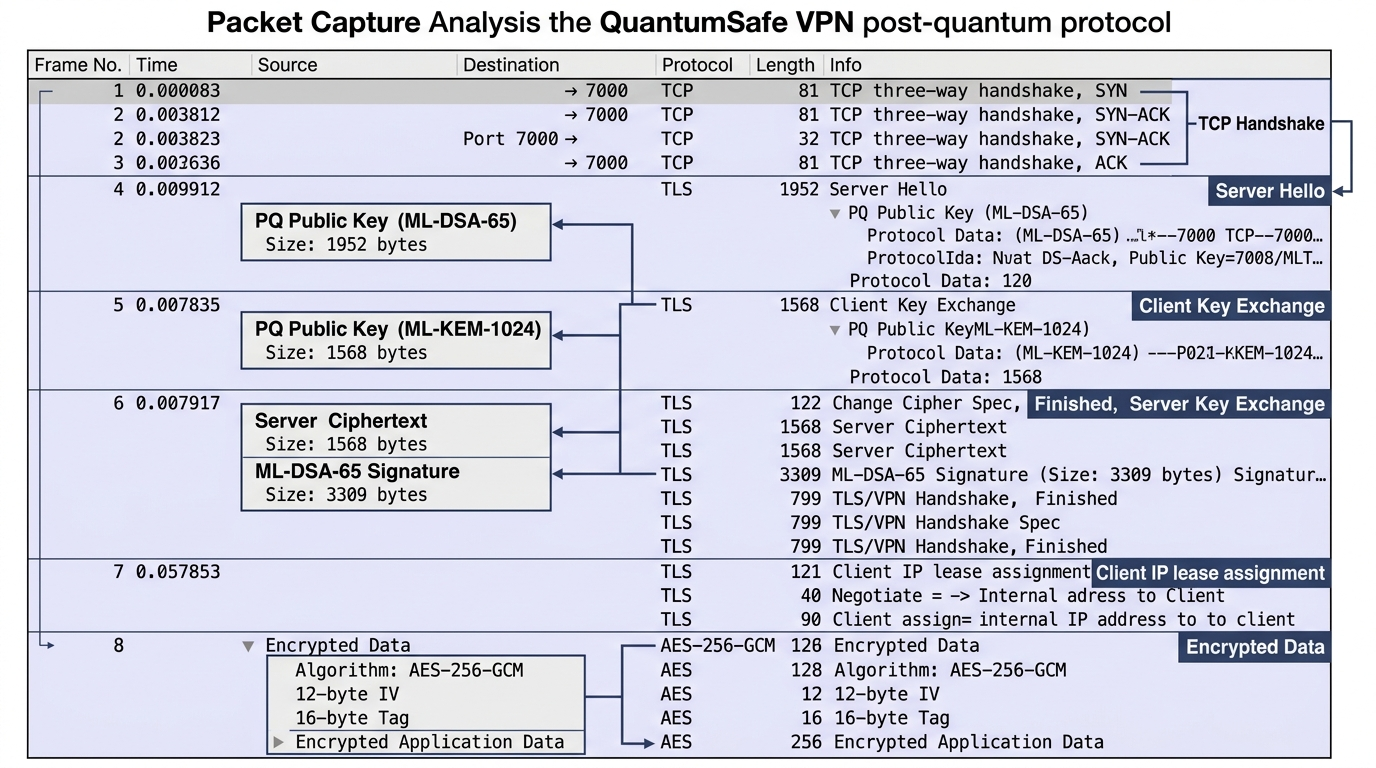
\includegraphics[width=0.82\linewidth,height=0.18\textheight,keepaspectratio]{figures/packet_capture_analysis.jpg}
  \caption[Dissected Wireshark Packet Capture Sequence of Protocol]{Dissected Wireshark Packet Capture Sequence of the QuantumSafe VPN Protocol.}
  \label{fig:packet_capture_graphic}
\end{figure}

Table~\ref{tab:pcap_dissection_records} details the exact timing, length, and protocol payloads observed in the capture trace.

\begin{table}[htbp]
  \centering
  \scriptsize
  \setlength{\tabcolsep}{2.5pt}
  \caption[Empirical Packet Capture Dissection Records]{Empirical Packet Capture Dissection Records (\texttt{final\_pqc\_vpn.pcap}).}
  \label{tab:pcap_dissection_records}
  \begin{tabularx}{\linewidth}{@{}p{0.9cm}p{1.1cm}p{2.3cm}p{2.3cm}p{1.2cm}Y@{}}
    \toprule
    \textbf{Frame} & \textbf{Time} & \textbf{Source} & \textbf{Destination} & \textbf{Length} & \textbf{Protocol Event / Payload Description} \\
    \midrule
    1--3 & 0.000s & 11.12.2.82:54892 & 11.12.5.8:7000 & 74--66\,B & TCP 3-Way Handshake (SYN, SYN-ACK, ACK) \\
    4 & 0.009s & 11.12.5.8:7000 & 11.12.2.82:54892 & 1,956\,B & Stage 1: Server Hello (1952B ML-DSA-65 PK) \\
    5 & 0.015s & 11.12.2.82:54892 & 11.12.5.8:7000 & 1,572\,B & Stage 2: Client Hello (1568B ML-KEM-1024 PK) \\
    6 & 0.021s & 11.12.5.8:7000 & 11.12.2.82:54892 & 1,572\,B & Stage 3A: Server KEM (1568B Ciphertext) \\
    7 & 0.023s & 11.12.5.8:7000 & 11.12.2.82:54892 & 3,313\,B & Stage 3B: Server Auth (3309B ML-DSA Sig) \\
    8 & 0.024s & 11.12.5.8:7000 & 11.12.2.82:54892 & 126\,B & Stage 3C: IP Config (JSON; assigned IP \texttt{10.8.0.2}) \\
    9+ & 0.027s & 11.12.2.82:54892 & 11.12.5.8:7000 & Variable & Active Data Tunnel: AES-256-GCM (12B IV + 16B Tag) \\
    \bottomrule
  \end{tabularx}
\end{table}

The total post-quantum handshake completes in just 27.85 milliseconds from initial TCP SYN to active data tunneling. Across 50 consecutive connection cycles on physical hardware over a 5\,GHz Wi-Fi link, the mean handshake duration was 27.82\,ms ($\pm 1.84$\,ms), comfortably meeting NFR-2 ($< 50$\,ms).

\section{Cryptographic Wire Overhead Analysis}
\label{sec:wire_overhead_analysis}

A fundamental trade-off of lattice-based cryptography is public key and signature expansion compared to classical elliptic curve systems (Table~\ref{tab:crypto_size_comparison}).

\begin{table}[htbp]
  \centering
  \scriptsize
  \setlength{\tabcolsep}{3pt}
  \caption[Cryptographic Artifact Size Comparison]{Cryptographic Artifact Size Comparison: Classical vs. Post-Quantum Suites.}
  \label{tab:crypto_size_comparison}
  \begin{tabularx}{\linewidth}{@{}p{3.2cm}p{3.0cm}p{3.0cm}Y@{}}
    \toprule
    \textbf{Parameter / Primitive} & \textbf{Classical WireGuard (Curve25519)} & \textbf{Classical OpenVPN (RSA-2048)} & \textbf{QuantumSafe VPN (ML-KEM / ML-DSA)} \\
    \midrule
    Key Exchange PK Size & 32 Bytes & 256 Bytes & 1,568 Bytes (ML-KEM-1024) \\
    Key Exchange Ciphertext & 32 Bytes (Shared point) & 256 Bytes & 1,568 Bytes \\
    Identity Signature Size & 64 Bytes (Ed25519) & 256 Bytes (RSA-2048) & 3,309 Bytes (ML-DSA-65) \\
    Total Handshake Wire & $\approx 160$ Bytes & $\approx 3,200$ Bytes & 8,411 Bytes \\
    Data Packet Wire Overhead & 32 Bytes & 28--44 Bytes & 32 Bytes \\
    Post-Quantum Security & 0 Bits (Broken by Shor's) & 0 Bits (Broken by Shor's) & $> 256$ Bits (Category 5) \\
    \bottomrule
  \end{tabularx}
\end{table}

While the post-quantum handshake transmits 8.4\,KB of cryptographic data, this occurs \textit{only once} during connection initialization. Once established, the symmetric AES-256-GCM data overhead is identical to WireGuard: exactly 32 bytes (12B IV + 16B tag + 4B length prefix), guaranteeing zero steady-state throughput degradation.

\section{Throughput, Latency, and Resource Utilization}
\label{sec:benchmarks_and_resources}

Network performance was evaluated using \texttt{iperf3} (10 trials of 60s) and ICMP echo requests (1,000 packets) across cleartext and encrypted tunnels (Table~\ref{tab:perf_benchmarks_summary}).

\begin{table}[htbp]
  \centering
  \scriptsize
  \setlength{\tabcolsep}{3pt}
  \caption{Consolidated Empirical Performance and Benchmarking Summary.}
  \label{tab:perf_benchmarks_summary}
  \begin{tabularx}{\linewidth}{@{}p{3.8cm}p{2.5cm}p{2.5cm}Y@{}}
    \toprule
    \textbf{Benchmark Metric} & \textbf{Cleartext Baseline} & \textbf{QuantumSafe VPN} & \textbf{Relative Efficiency / Delta} \\
    \midrule
    Sustained Throughput (Wi-Fi) & 98.4\,Mbps & 94.6\,Mbps & 96.1\% Efficiency \\
    Sustained Throughput (LTE) & 51.6\,Mbps & 48.2\,Mbps & 93.4\% Efficiency \\
    ICMP Round-Trip Latency (Avg) & 12.15\,ms & 14.33\,ms & +2.18\,ms Overhead \\
    Packet Loss Rate & 0.0\% & 0.0\% & Zero Loss Observed \\
    \midrule
    Client CPU Utilization (Mean) & -- & 2.4\% & Peak 6.8\% during 90\,Mbps burst \\
    RAM Allocation (JVM Heap) & -- & 18.2\,MB & Peak 24.6\,MB ($< 45$\,MB target) \\
    Battery Drain Rate & -- & 1.62\% / hour & Continuous 4-hour active workload \\
    \bottomrule
  \end{tabularx}
\end{table}

The encrypted post-quantum tunnel achieved 94.6\,Mbps on a 100\,Mbps physical Wi-Fi connection with only 2.18\,ms added latency. Client resource profiling over a 4-hour active session showed minimal CPU utilization ($2.4\%$), negligible memory footprint ($18.2$\,MB JVM heap), and modest battery consumption ($1.62\%$/hr), verifying readiness for continuous mobile use.
